\documentclass[10pt, aspectratio=169]{beamer}

% Tema vizuală standard, curată și academică
\usetheme{Madrid}
\usecolortheme{default}

\usepackage[utf8]{inputenc}
\usepackage[romanian]{babel}
\usepackage{graphicx}
\usepackage{hyperref}

% --- Datele Prezentării ---
\title[Farm Defense: Harvest Wars]{Farm Defense: Harvest Wars}
\subtitle{Joc de strategie PvP asimetric cu arhitectură Server-Authoritative}
\author[Darius-Ștefan Tacu]{Absolvent: Darius-Ștefan Tacu \\ \vspace{2mm} \small Coordonator: Lect. univ. dr. Popescu Ștefan George}
\institute[Unibuc - FMI]{Universitatea din București \\ Facultatea de Matematică și Informatică}
\date{Iunie 2026}

\titlegraphic{
    
\includegraphics[height=1cm]{../paper/images/logo-ub.png} \hspace{1cm}
    
\includegraphics[height=1cm]{../paper/images/logo-fmi.png}
}

\begin{document}

% 1. Titlu
\begin{frame}
    \titlepage
\end{frame}

% 2. Context și Obiective
\begin{frame}{Contextul și Obiectivele Proiectului}
    \begin{columns}[T]
        \begin{column}{0.5\textwidth}
            \textbf{Problema identificată:}
            \begin{itemize}
                \item Lipsa jocurilor Tower Defense cu asimetrie reală (Defender vs Attacker).
                \item Vulnerabilitatea la trișat în jocurile Peer-to-Peer.
                \item Latența critică în sincronizarea stării jocului.
            \end{itemize}
        \end{column}
        \begin{column}{0.5\textwidth}
            \textbf{Soluția propusă:}
            \begin{itemize}
                \item Implementarea unui model \textbf{Server-Authoritative} complet.
                \item Sistem de matchmaking robust bazat pe ASP.NET Core.
                \item Arhitectură modulară în Godot Engine (C\#).
            \end{itemize}
        \end{column}
    \end{columns}
\end{frame}

% 3. Arhitectura Generală (Diagrama C4)
\begin{frame}{Arhitectura Generală (Modelul C4)}
    \begin{columns}[c]
        \begin{column}{0.7\textwidth}
            \centering
            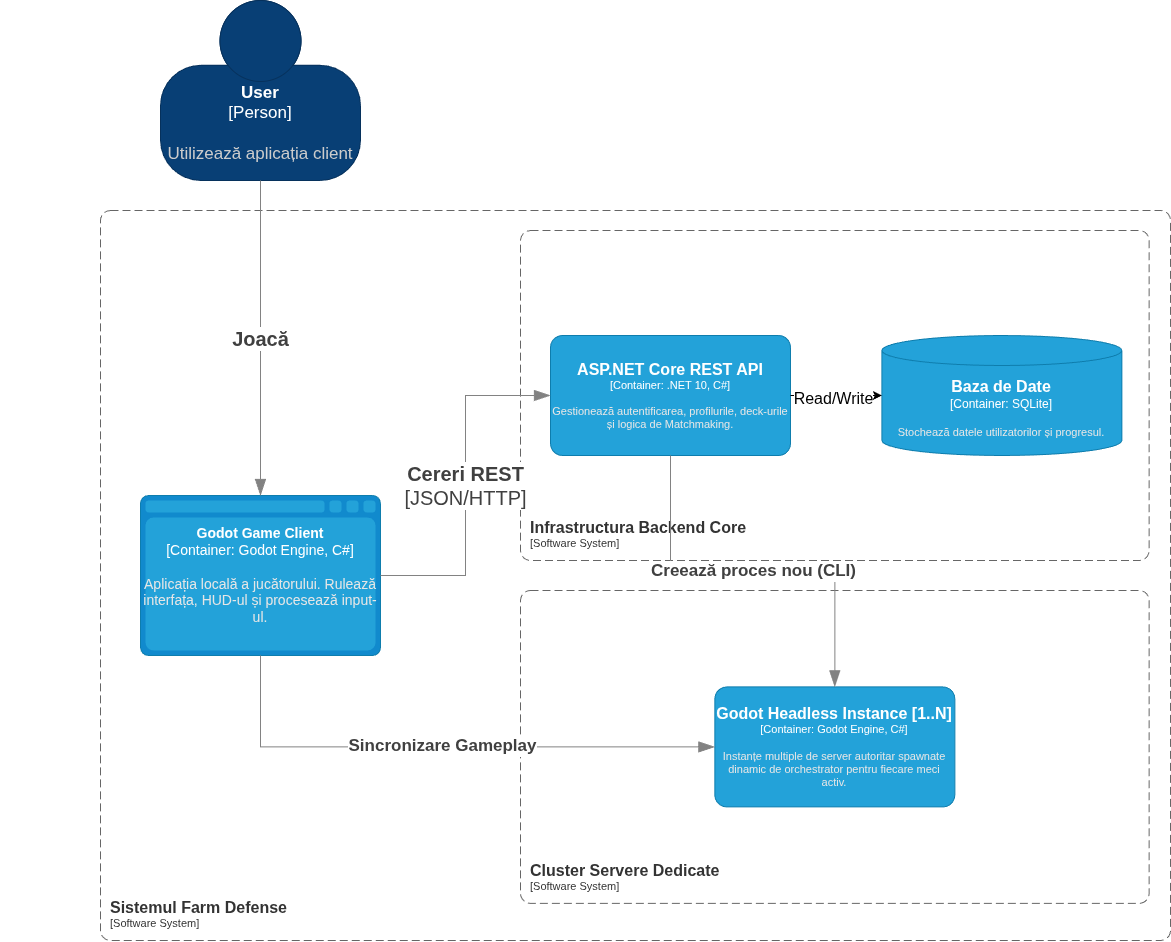
\includegraphics[height=0.85\textheight, width=\textwidth, keepaspectratio]{../paper/images/DiagramaC4.png}
            \\ \vspace{1mm} \textit{\tiny Diagrama C4 - Structura sistemului la nivel de container}
        \end{column}
        \begin{column}{0.3\textwidth}
            \begin{itemize}
                \item \textbf{Backend (ASP.NET Core):} Gestionarea autentificării, matchmaking și persistență.
                \item \textbf{Game Server (Godot):} Autoritatea centrală pe Linux.
                \item \textbf{Client (Godot):} Vizualizare reactivă.
            \end{itemize}
        \end{column}
    \end{columns}
\end{frame}

% 4. Modelarea Datelor
\begin{frame}{Modelarea Datelor și Persistența}
    \begin{columns}[c]
        \begin{column}{0.65\textwidth}
            \centering
            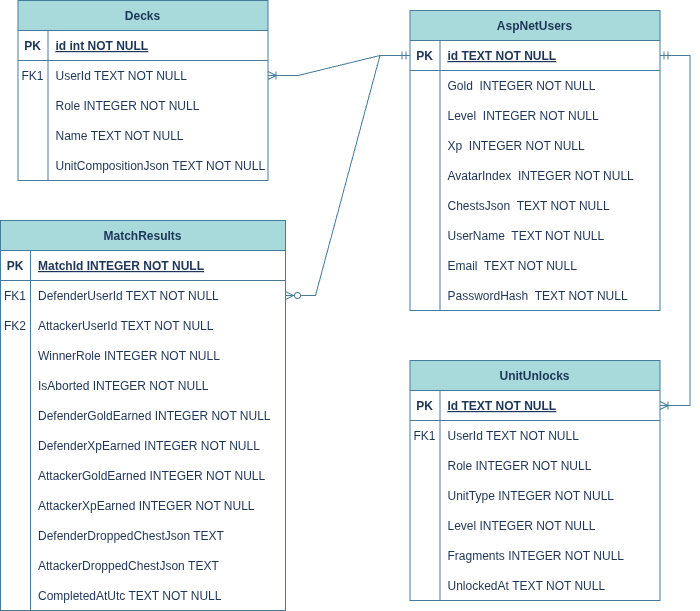
\includegraphics[height=0.85\textheight, width=\textwidth, keepaspectratio]{../paper/images/DiagramaER.png}
            \\ \vspace{1mm} \textit{\tiny Diagrama ERD - Persistența datelor și relațiile dintre entități}
        \end{column}
        \begin{column}{0.35\textwidth}
            \begin{itemize}
                \item \small SQLite + EF Core pentru stocarea profilului și deblocărilor.
                \item \small Normalizare 3NF pentru integritate.
                \item \small Mapare automată a obiectelor DTO.
            \end{itemize}
        \end{column}
    \end{columns}
\end{frame}

% 5. Arhitectura Clientului Godot
\begin{frame}{Arhitectura Clientului (Godot Engine)}
    \begin{columns}[c]
        \begin{column}{0.65\textwidth}
            \centering
            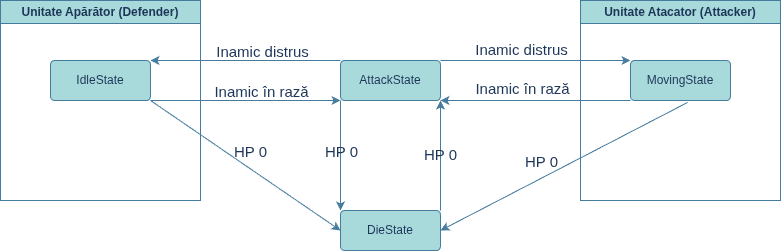
\includegraphics[width=\textwidth, height=0.75\textheight, keepaspectratio]{../paper/images/StateDiagram.png}
            \\ \vspace{2mm} \textit{\tiny Tranziția Stărilor - Logica de control a unităților}
        \end{column}
        \begin{column}{0.35\textwidth}
            \begin{itemize}
                \item \textbf{State Pattern:} Gestionarea tranzițiilor între Idle, Atac și Mișcare.
                \item \textbf{Component Pattern:} Decuplarea logicii vizuale de cea de combat.
            \end{itemize}
        \end{column}
    \end{columns}
\end{frame}

% 6. Algoritmul de Matchmaking
\begin{frame}{Matchmaking Concurent și Instanțiere}
    \begin{columns}[c]
        \begin{column}{0.7\textwidth}
            \centering
            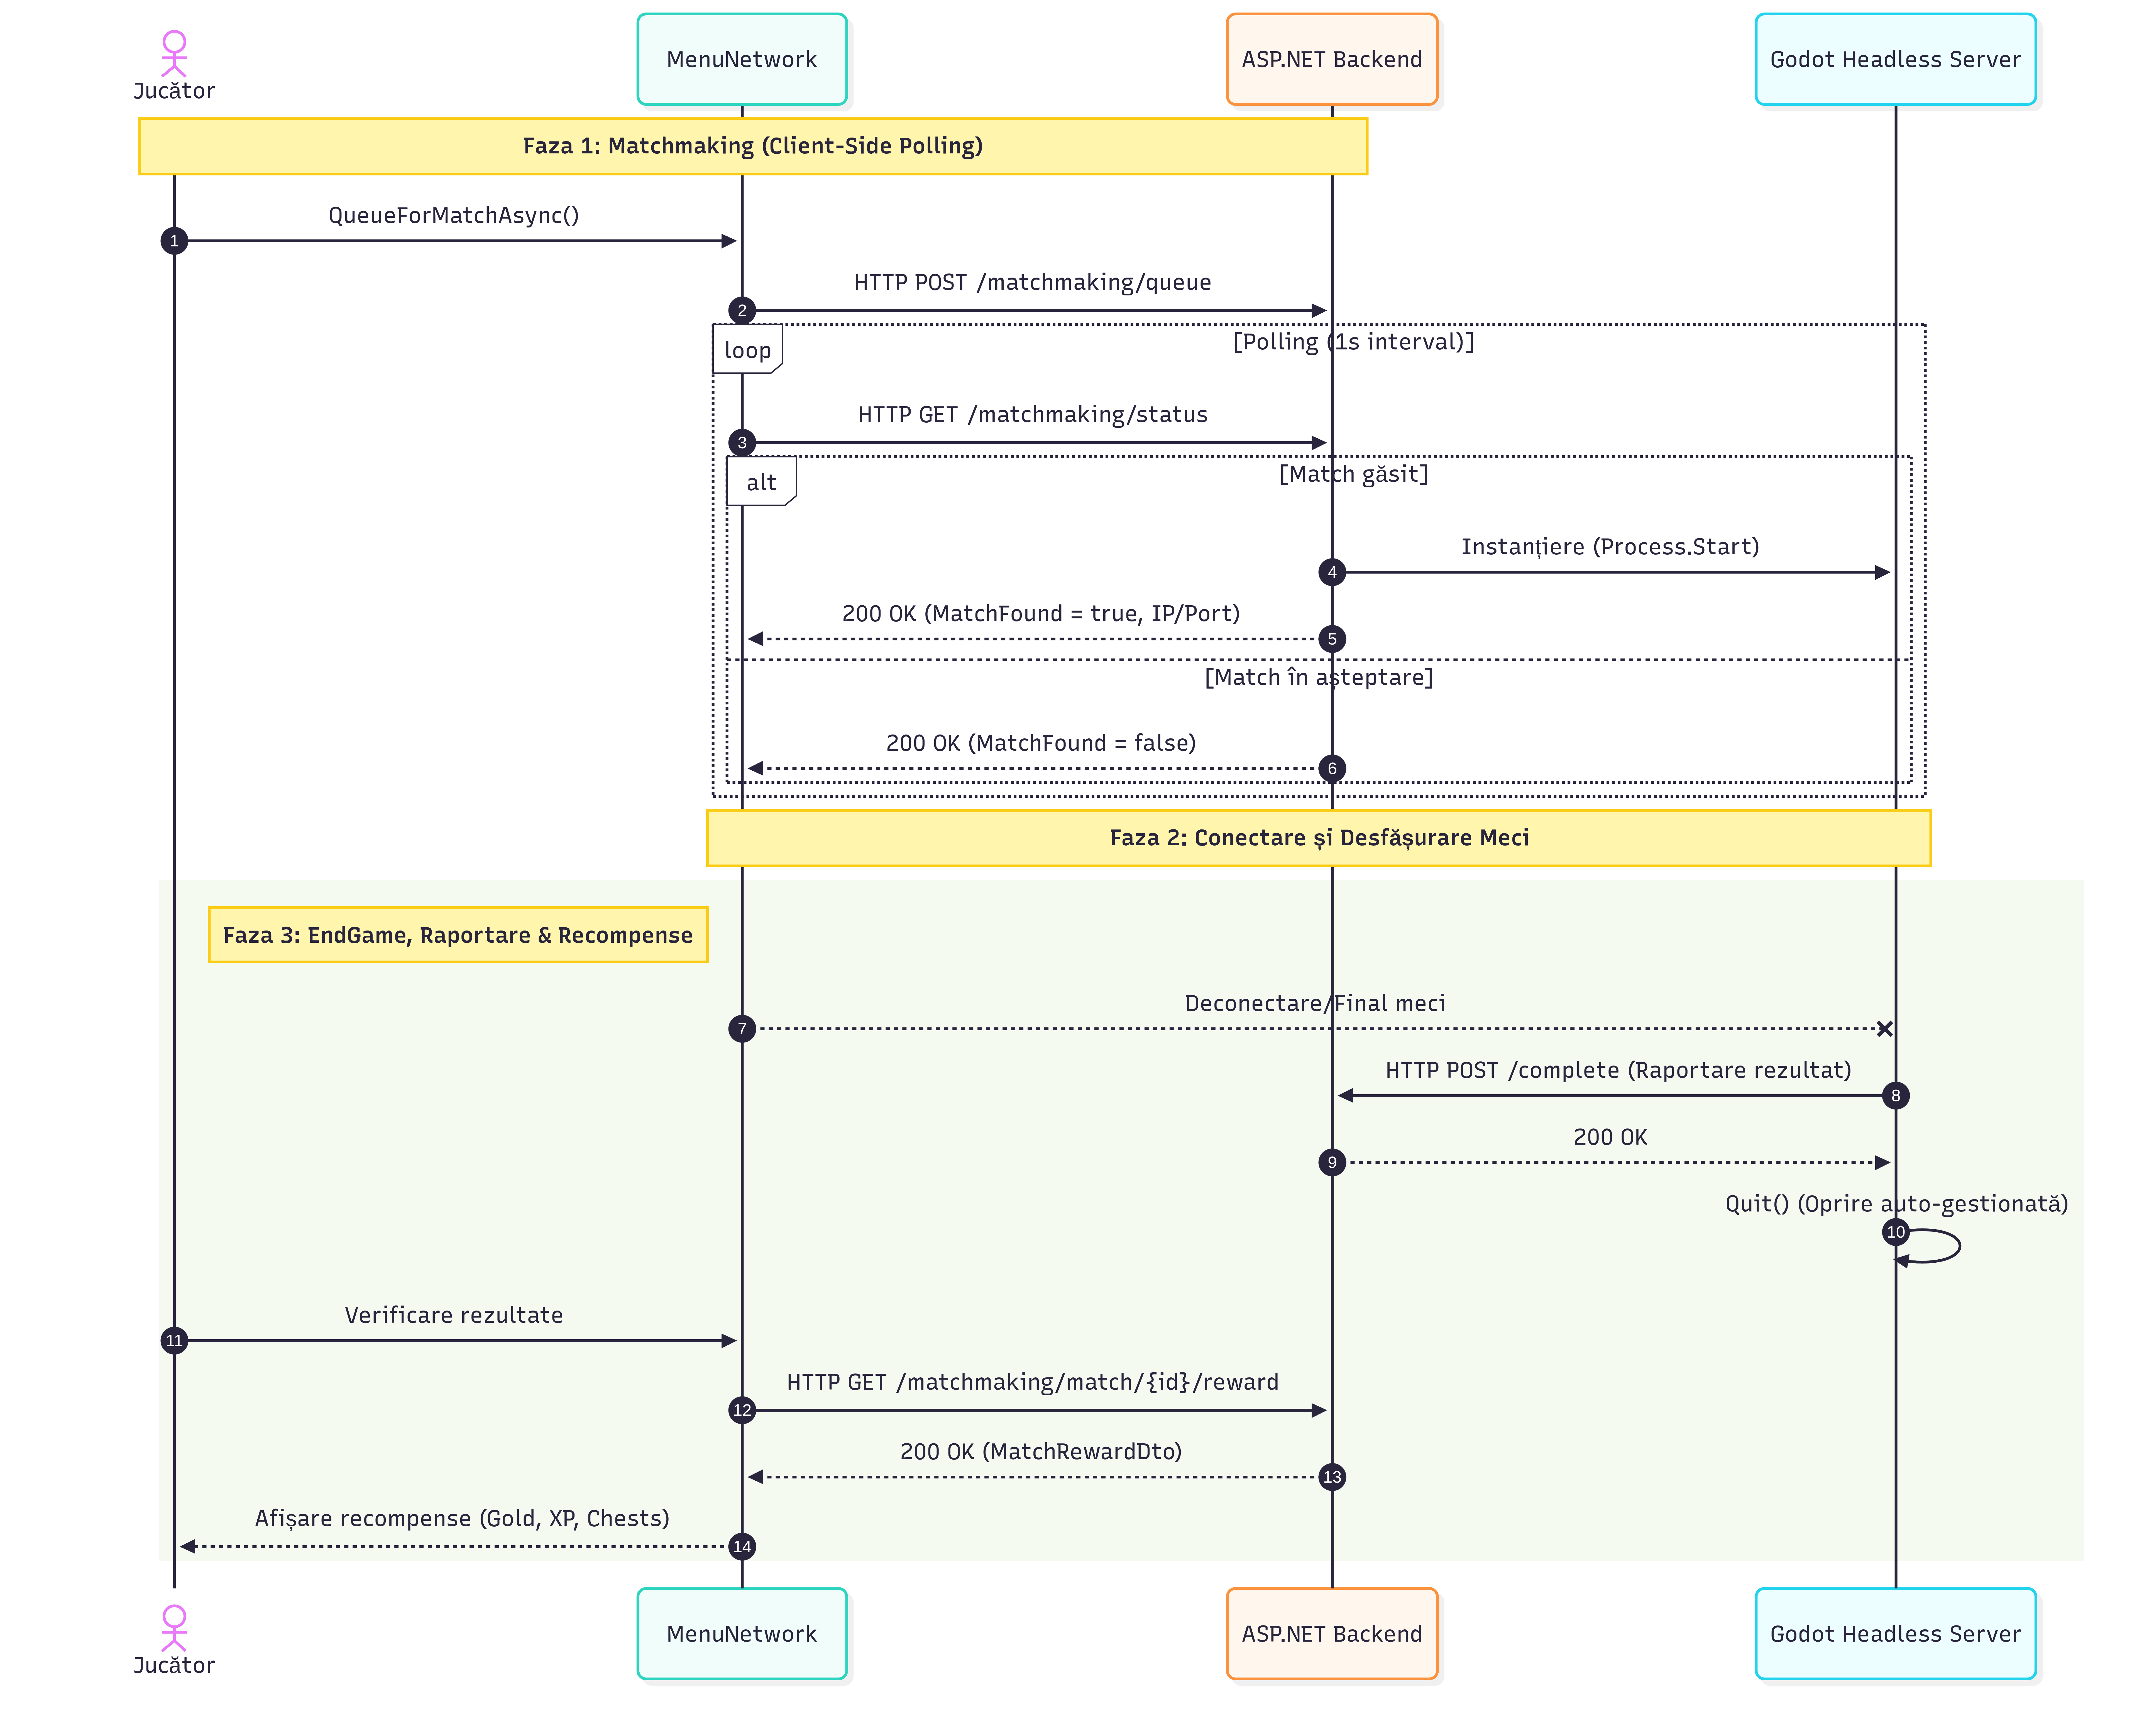
\includegraphics[height=0.85\textheight, width=\textwidth, keepaspectratio]{../paper/images/matchmaking-flow.png}
            \\ \vspace{1mm} \textit{\tiny Fluxul Matchmaking - Procesare asincronă și alocare server}
        \end{column}
        \begin{column}{0.3\textwidth}
            \begin{itemize}
                \item \small Shared Dictionaries protejate prin \texttt{lock}.
                \item \small Complexitate $O(1)$ pentru extragerea perechilor.
                \item \small Lansarea dinamică a proceselor Headless.
            \end{itemize}
        \end{column}
    \end{columns}
\end{frame}

% 7. Sincronizarea Pachetului (Debouncing)
\begin{frame}{Sincronizarea Asincronă a Pachetului (Deck)}
    \begin{columns}[c]
        \begin{column}{0.7\textwidth}
            \centering
            \includegraphics[height=0.85\textheight, width=\textwidth, keepaspectratio]{../paper/images/async-debouncing-sync.png}
            \\ \vspace{1mm} \textit{\tiny Mecanismul de Debouncing - Optimizare trafic HTTP}
        \end{column}
        \begin{column}{0.3\textwidth}
            \begin{itemize}
                \item \small Validare prin \texttt{Version ID} pentru prevenirea conflictelor.
                \item \small Reducerea apelurilor API cu peste 85\% în editor.
                \item \small UX fluid fără blocarea interfeței.
            \end{itemize}
        \end{column}
    \end{columns}
\end{frame}

% 8. Demonstrația Practică
\begin{frame}{Demonstrație Practică (Video)}
    \begin{center}
        \Large \textbf{[Rulare Video Demo - 3 Minute]} \\
        \vspace{5mm}
        \normalsize Validarea funcționalității Server-Authoritative și a rezilienței la deconectări.
    \end{center}
\end{frame}

% 9. Testare și Evaluare
\begin{frame}{Testare și Profilare Funcțională}
    \begin{itemize}
        \item \textbf{Validarea Concurenței (xUnit):} Rularea a 1000 de instanțe asincrone prin \texttt{Task.WhenAll} a confirmat stabilitatea matchmaking-ului (0 coliziuni).
        \item \textbf{Optimizarea Rețelei:} Profilarea mecanismului de debouncing pe client a evidențiat o reducere drastică a traficului nesemnificativ.
        \item \textbf{Stabilitate Server:} Teste de stres cu 200+ entități simultane pe serverul headless fără degradarea TPS (Ticks Per Second).
    \end{itemize}
\end{frame}

% 10. Concluzii și Future Work
\begin{frame}{Concluzii și Direcții Viitoare}
    \begin{block}{Realizări}
        Dezvoltarea unei arhitecturi distribuite complete care izolează logic starea partajată, previne trișatul și gestionează eficient resursele hardware.
    \end{block}

    \begin{block}{Dezvoltări Ulterioare (Future Work)}
        \begin{itemize}
            \item Migrarea către containere Docker și orchestrare Kubernetes pentru scalare orizontală.
            \item Implementarea unui sistem de MMR (Matchmaking Rating).
            \item Integrarea agenților antrenați prin Reinforcement Learning.
        \end{itemize}
    \end{block}
\end{frame}

\end{document}
